\begin{figure}[!b]
\begin{subfigure}{0.495\textwidth}
\centering
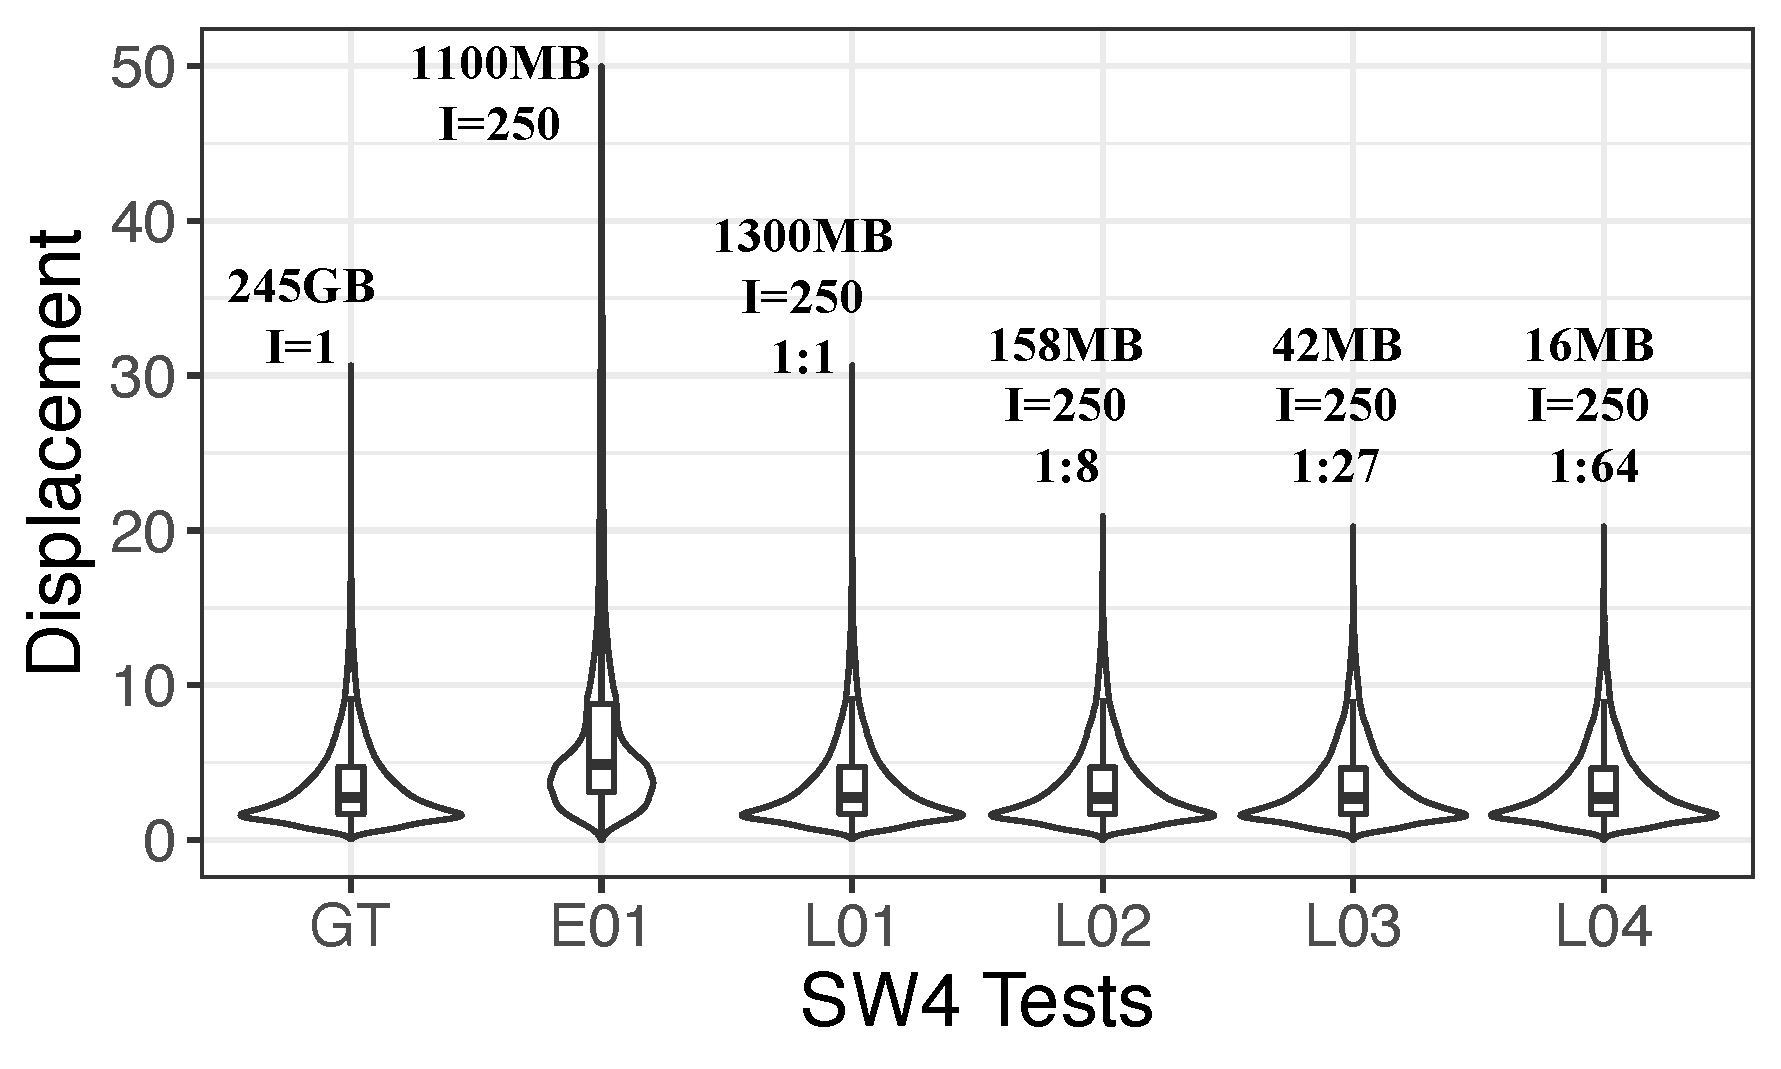
\includegraphics[width=\linewidth]{Images/sw4_violinplot1.pdf}
\vspace{-5mm}
\caption{High displacement near the epicenter.}
\label{fig:epicenter}
\end{subfigure}
\begin{subfigure}{0.495\textwidth}
\centering
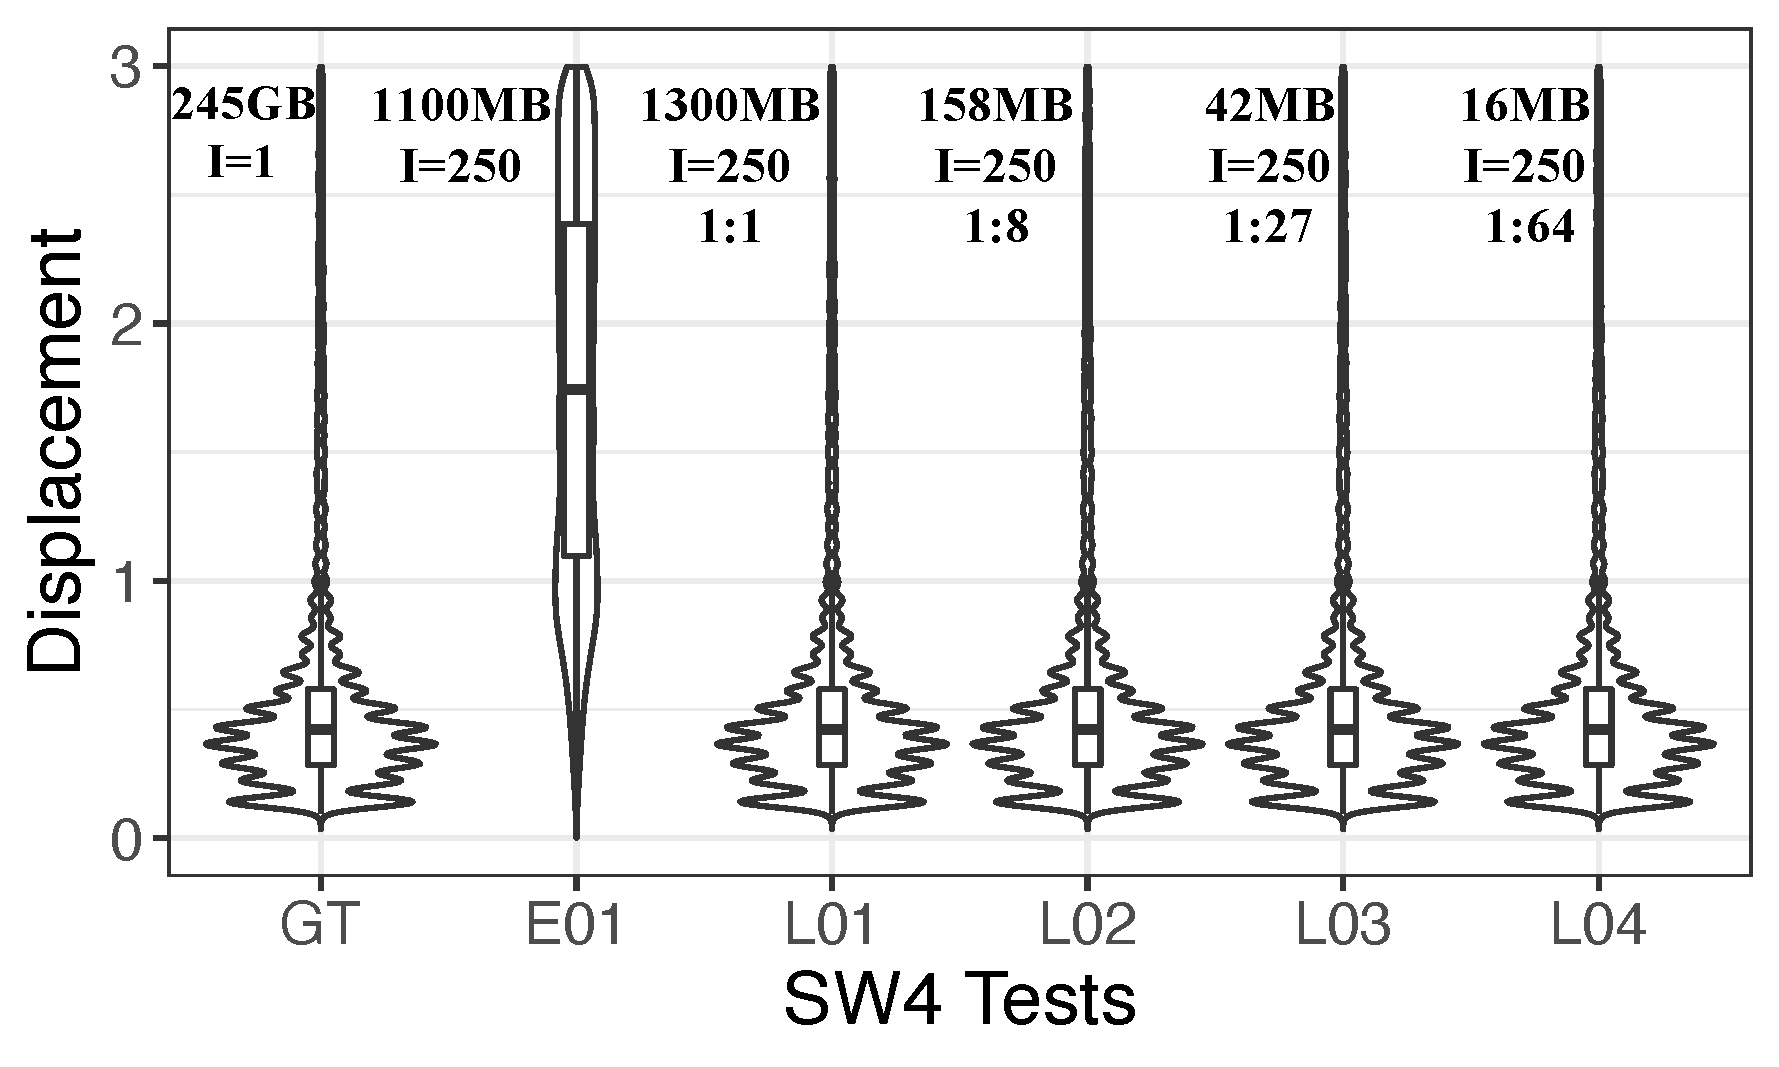
\includegraphics[width=\linewidth]{Images/sw4_violinplot2.pdf}
\vspace{-5mm}
\caption{Low displacement away from the epicenter.}
\label{fig:clusters}
\end{subfigure}
\vspace{-2mm}
\caption{Violin plots of the distribution of particle displacement for the ground truth (GT), one Eulerian configuration and four Lagrangian configurations. The Eulerian configuration, with access to a limited number of time slices, overestimates the displacement. The Lagrangian representation captures displacement in both settings, in regions near and away from the epicenter, accurately.}
\vspace{-5mm}
\label{fig:sw4_violinplot}
\end{figure}
